\section{{\cjkfont 无序跳跃输运与温度依赖：反偏机理比较的共同基础}\allowbreak{}}\label{sec:transport-temperature}
\subsection{{\cjkfont 本章的结论与阅读范围}\allowbreak{}}
{\cjkfont 有机半导体的迁移率本身对温度、载流子占据和电场敏感。因此，端口反向电流的温度依赖不能直接等同于某个产生步骤的激活能。我们将无序跳跃输运设为不同反偏候选机制的共同基础，再比较陷阱辅助产生、}\allowbreak{}Coulomb {\cjkfont 型}\allowbreak{} Poole--Frenkel{\cjkfont （}\allowbreak{}PF{\cjkfont ）发射、供受体对循环和接触供给。这样，同一套输运假设下的差异才主要反映所比较的机制。}\allowbreak{}

{\cjkfont 本章首先说明这个选择的物理含义，再介绍高斯态密度、迁移率与扩散的共同闭合，随后报告已完成的数值检查和文献读图。最后讨论接触区暴露出来的适用域问题。后续章节保留早期探索：其中固定迁移率、单能级储库以及有限图电流均应按原有条件理解，不能自动升级为本章无序输运框架下的器件预测。}\allowbreak{}

{\cjkfont 截至本次修订，两个明确接触情景的完整器件变温计算已通过网格与守恒核验。其温度响应显著强于文献，且主要由接触泄漏控制。原近欧姆接触情景的高占据适用域问题仍未解决。本章保留这项失败对照，并新增完整温度预测、来源分账及独立材料参数比较。}\allowbreak{}

\subsection{{\cjkfont 局域跳跃与}\allowbreak{} PF {\cjkfont 不是同一件事}\allowbreak{}}
{\cjkfont 局域跳跃描述载流子在空间上局域的电子态之间转移。其速率可采用}\allowbreak{} Miller--Abrahams{\cjkfont 、}\allowbreak{}Marcus {\cjkfont 或包含量子振动的}\allowbreak{} MLJ {\cjkfont 等不同近似，分别对应不同的核与能量交换假设。载流子沿许多这样的跃迁穿过无序网络，宏观上才表现为迁移率。}\allowbreak{}

{\cjkfont 经典}\allowbreak{} Coulomb {\cjkfont 型}\allowbreak{} PF {\cjkfont 则描述电场降低带电中心对逸出载流子的吸引势垒。在无限程连续介质近似中，降垒随电场平方根增长。它是一种发射势垒的物理机制，既不等于所有跳跃，也不等于任何经验上呈现平方根场依赖的迁移率。无序迁移率的场依赖有时也被称为}\allowbreak{}“PF {\cjkfont 型}\allowbreak{}”{\cjkfont ，但这是函数形状的命名，不能证明存在同一个}\allowbreak{} Coulomb {\cjkfont 降垒过程。}\allowbreak{}

{\cjkfont 陷阱辅助隧穿与跳跃输运可以共存：前者可能决定电子}\allowbreak{}--{\cjkfont 空穴对怎样进入可输运态，后者决定生成后的载流子怎样被搬运和收集。不过，若某个陷阱发射已经作为同一微观网络的一条跃迁计算，就不能再把它完整地加入独立}\allowbreak{} PF {\cjkfont 或}\allowbreak{} TAT {\cjkfont 产生项。共同基础的关键是定义状态和过程边界，避免重复计数。}\allowbreak{}

\begin{figure}[htbp]\centering
\begin{tikzpicture}[node distance=8mm,box/.style={draw=tolblue,rounded corners,align=center,text width=3.3cm,minimum height=1.2cm,font=\small},>=Stealth]
\node[box](g){{\cjkfont 产生与复合}\allowbreak{}\\PF{\cjkfont 、}\allowbreak{}TAT{\cjkfont 、供受体循环}\allowbreak{}};
\node[box,right=of g](t){{\cjkfont 无序跳跃输运}\allowbreak{}\\$\mu(n,F,T)$ {\cjkfont 与扩散}\allowbreak{}};
\node[box,right=of t](c){{\cjkfont 电极边界}\allowbreak{}\\{\cjkfont 注入、抽取、界面占据}\allowbreak{}};
\draw[<->](g)--(t);\draw[<->](t)--(c);
\node[box,below=10mm of t,text width=7.1cm](p){Poisson {\cjkfont 与连续性方程}\allowbreak{}\\{\cjkfont 电场、占据、准费米能级和电流共同求解}\allowbreak{}};
\draw[<->](g.south)--(p.west);\draw[<->](t)--(p);\draw[<->](c.south)--(p.east);
\end{tikzpicture}
\caption{{\cjkfont 共同器件框架的概念示意。箭头表示自洽反馈，不代表可直接相加的独立电流。图不包含材料拟合结果。}\allowbreak{}}\label{fig:common-framework}
\end{figure}

\subsection{{\cjkfont 从高斯态密度到载流子占据}\allowbreak{}}
{\cjkfont 无序材料中，不同局部环境对应不同位点能量。作为可检验的工作近似，对电子或空穴输运流形分别使用高斯态密度}\allowbreak{}
\begin{equation}
 g(\varepsilon)=\frac{N}{\sqrt{2\pi}\sigma}\exp\!\left[-\frac{(\varepsilon-\varepsilon_0)^2}{2\sigma^2}\right],\qquad
 n=\int g(\varepsilon)f(\varepsilon,E_F,T)\,d\varepsilon .
\end{equation}
{\cjkfont 这里}\allowbreak{} $N$ {\cjkfont 是位点密度，}\allowbreak{}$\sigma$ {\cjkfont 是能量无序宽度，}\allowbreak{}$E_F$ {\cjkfont 为局域准费米能级。电子的}\allowbreak{} $f$ {\cjkfont 取}\allowbreak{} Fermi {\cjkfont 占据；空穴采用相应空态占据和一致的能量符号。单一平均能级的占据率不能替代整个}\allowbreak{} DOS {\cjkfont 的积分。}\allowbreak{}

{\cjkfont 低密度时，载流子倾向占据深尾态，离开这些态需要较大的热激活代价。密度增加时，深尾态被部分填满，可参与输运的能量窗口改变。因而迁移率可以依赖密度；但这不意味着载流子必须在同一时刻占据一条连续分子链。电流是随时间发生的跳跃序列，路径瓶颈取决于能量、距离、占据和网络连通性。}\allowbreak{}

{\cjkfont 将}\allowbreak{} $N=a^{-3}$ {\cjkfont 用于规则格点模型时，}\allowbreak{}$a$ {\cjkfont 是该模型的位点间距。它不应同时被随意解释为化学分子直径、真实相区尺度、陷阱到受体的跃迁距离或所有模型共用的拟合长度。}\allowbreak{}

\subsection{{\cjkfont 迁移率与扩散必须使用同一统计闭合}\allowbreak{}}
{\cjkfont 本轮体输运采用}\allowbreak{} Pasveer {\cjkfont 等的高斯无序迁移率参数化，写为}\allowbreak{}
\begin{equation}
 \mu(n,F,T)=\mu_*\exp[-0.42s^2]g_1(c,s)g_2(u,s),\qquad
 s=\frac{\sigma}{k_BT},\quad c=na^3,\quad u=\frac{q|F|a}{\sigma}.
\end{equation}
$\mu_*$ {\cjkfont 为温度无关的前因子；采用}\allowbreak{} SI {\cjkfont 能量单位时}\allowbreak{} $u$ {\cjkfont 中显式包含}\allowbreak{} $q${\cjkfont 。原参数化的密度与场因子为}\allowbreak{}
\begin{align}
 g_1&=\exp\!\left[\tfrac12(s^2-s)(2c)^\delta\right], &
 \delta&=\frac{2\{\ln(s^2-s)-\ln(\ln4)\}}{s^2},\\
 g_2&=\exp\!\left[0.44(s^{3/2}-2.2)\bigl(\sqrt{1+0.8u^2}-1\bigr)\right].
\end{align}
{\cjkfont 这些式子是对规定无序格点主方程结果的参数化，不是任意材料、任意占据和电场下的定理。我们使用的文献比较窗口约为}\allowbreak{} $2\le s\le6${\cjkfont 、}\allowbreak{}$10^{-6}\le c\le10^{-2}${\cjkfont 。原图场范围到}\allowbreak{} $u\simeq3${\cjkfont ；图覆盖范围不能解释成普适有效性边界。高占据接触区尤其需要单独审查。}\allowbreak{}

{\cjkfont 相同}\allowbreak{} DOS {\cjkfont 的热力学压缩率同时决定广义}\allowbreak{} Einstein {\cjkfont 关系：}\allowbreak{}
\begin{equation}
 \frac{D}{\mu}=\frac{n}{q(\partial n/\partial E_F)_T}.
\end{equation}
{\cjkfont 此式中}\allowbreak{} $E_F$ {\cjkfont 以焦耳计。稀薄}\allowbreak{} Boltzmann {\cjkfont 极限恢复}\allowbreak{} $D/\mu=k_BT/q${\cjkfont 。在有限占据时，如果只修改迁移率而仍无条件使用稀薄}\allowbreak{} Einstein {\cjkfont 关系，就会把不同统计假设拼在一起。这里的关系仍依赖局域准平衡，强场下这一前提本身要检查。}\allowbreak{}

{\cjkfont 数值上使用逆活度型广义}\allowbreak{} Scharfetter--Gummel {\cjkfont 通量，并分别检查电子和空穴的符号。等准费米能级时电流精确为零、各面电流守恒，是最低要求；这些要求不等于接触模型已经真实。}\allowbreak{}

\begin{figure}[htbp]\centering
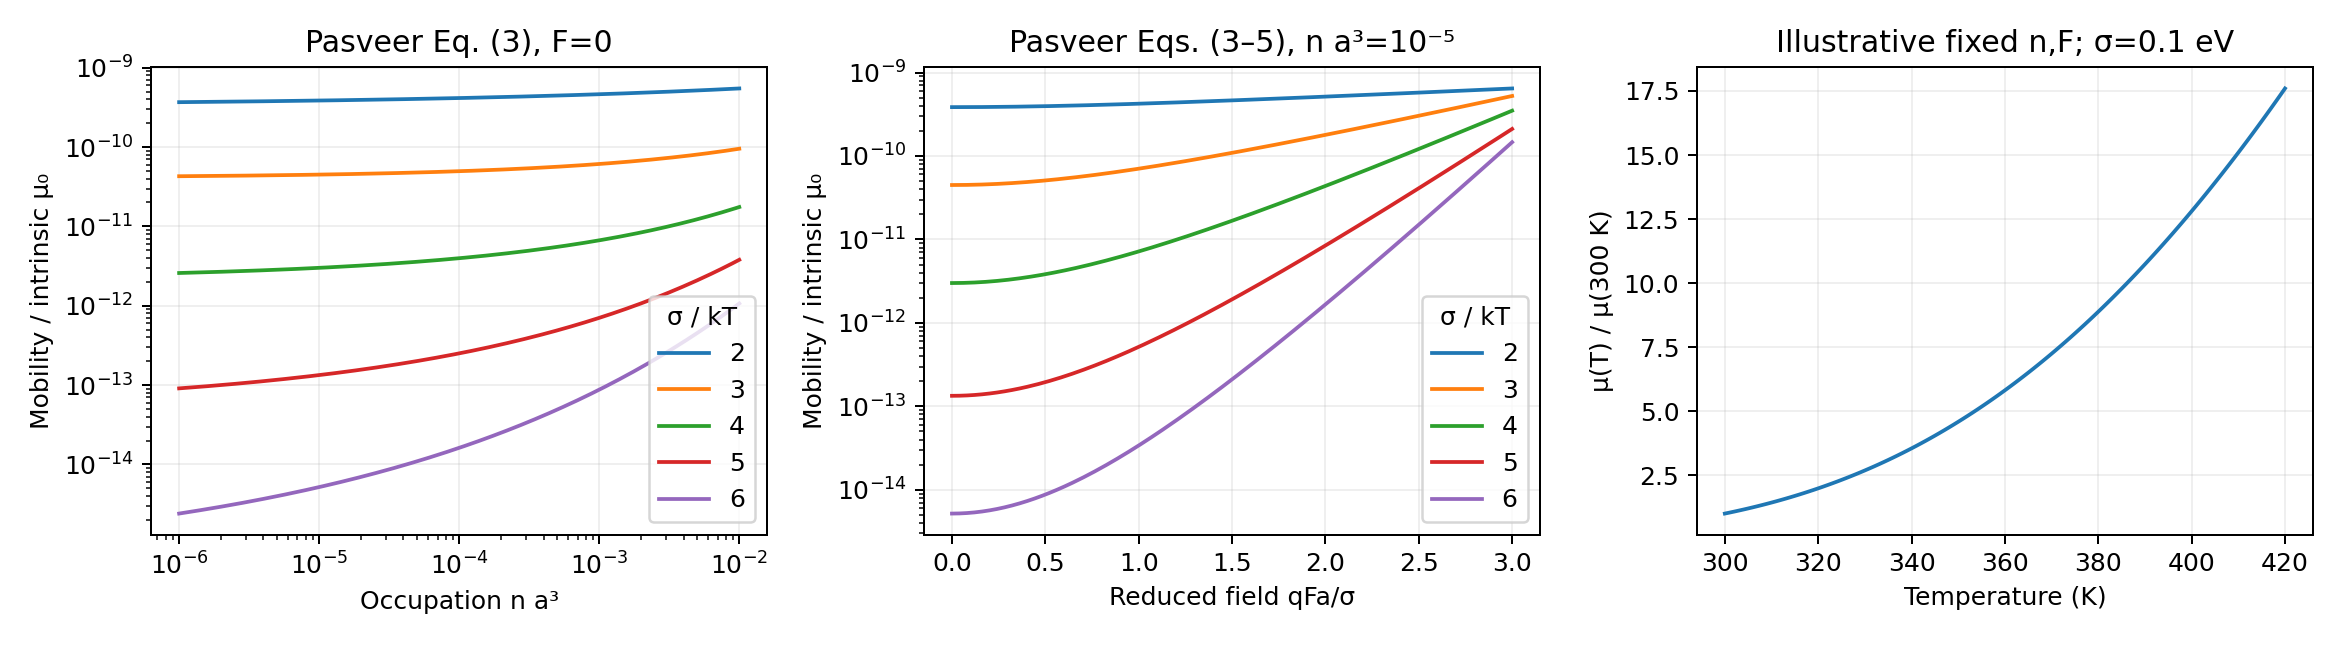
\includegraphics[width=.97\linewidth]{figures/temperature_transport_benchmark.png}
\caption{{\cjkfont 独立输运模块对已发表}\allowbreak{} Pasveer {\cjkfont 参数化的复现。它展示温度、占据与场的联合作用；不是重新计算原论文三维主方程数据，也不是}\allowbreak{} D18:L8-BO {\cjkfont 实测迁移率。}\allowbreak{}}\label{fig:transport-temperature-benchmark}
\end{figure}

\subsection{{\cjkfont 为什么端电流激活能不等于产生势垒}\allowbreak{}}
{\cjkfont 定义某一可观测量的局部表观激活能为}\allowbreak{}
\begin{equation}
 E_{a,\mathrm{app}}=-k_B\frac{\partial\ln |J|}{\partial(1/T)}.
\end{equation}
{\cjkfont 导数必须说明保持什么不变。固定端电压、固定平均场和固定局部场不是同一实验；随温度变化的空间电荷和接触势垒会重分配内部电压。}\allowbreak{}

{\cjkfont 在供给限制且充分收集的理想稳态极限，}\allowbreak{}$J\simeq q\int G\,dx${\cjkfont 。此时迁移率变化可以主要改变密度和渡越时间，而未必同比例改变电流。存在复合、有限抽取或空间电荷时，可形式上写出}\allowbreak{} $J\simeq qdG\eta_{\mathrm{coll}}${\cjkfont ，进而温度导数包含产生与收集两部分。这个分解也只有在均匀近似、分支定义明确且没有额外注入或倍增时才成立；一般器件应直接使用连续性分账。}\allowbreak{}

{\cjkfont 即便只看低密度低场迁移率，}\allowbreak{}$\ln\mu=\ln\mu_*-0.42(\sigma/k_BT)^2$ {\cjkfont 也不是恒定势垒的}\allowbreak{} Arrhenius {\cjkfont 直线。其局部温度导数对应}\allowbreak{} $E_{a,\mu}=0.84\sigma^2/(k_BT)${\cjkfont 。因此}\allowbreak{}“{\cjkfont 斜率随}\allowbreak{} $1/T$ {\cjkfont 变化}\allowbreak{}”{\cjkfont 不能单独证明某个产生机制是跳跃。}\allowbreak{}

{\cjkfont 经典}\allowbreak{} Marcus {\cjkfont 单步速率含}\allowbreak{} $T^{-1/2}$ {\cjkfont 前因子，且势垒为}\allowbreak{} $(\lambda+\Delta G)^2/(4\lambda)${\cjkfont 。若}\allowbreak{} $\Delta G$ {\cjkfont 包含线性场做功，势垒通常对场呈二次函数，只在有限场窗内近似线性。}\allowbreak{}MLJ {\cjkfont 多振动态求和、}\allowbreak{}DOS {\cjkfont 积分及速率串联会进一步改变表观斜率。}\allowbreak{}PF {\cjkfont 的热发射也可有很强的温度依赖；}\allowbreak{}CT {\cjkfont 场解离并不普遍等同于}\allowbreak{} Coulomb PF{\cjkfont 。不同机制的简短线性作图规则只能用作受限模型检查。}\allowbreak{}

\subsection{{\cjkfont 补充图}\allowbreak{} S10 {\cjkfont 提供了怎样的文献约束}\allowbreak{}}
Huang {\cjkfont 等补充图}\allowbreak{} S10 {\cjkfont 给出了}\allowbreak{} PM6:BTP-eC9 {\cjkfont 在}\allowbreak{} 300{\cjkfont 、}\allowbreak{}340{\cjkfont 、}\allowbreak{}380{\cjkfont 、}\allowbreak{}420 K {\cjkfont 的反向}\allowbreak{} $J$--$V${\cjkfont 。此前认为论文没有可用固定偏压变温电流的判断需要修正。我们对原图做了颜色、坐标和线宽核验后的数字化，结果见表。它们是读图估计，不是作者原始数据，也不是当前}\allowbreak{} D18:L8-BO {\cjkfont 样品的测量。}\allowbreak{}

\begin{table}[htbp]\centering\small
\begin{tabular}{rrrr}\toprule
$T$ (K)&$J(-5\,\mathrm V)$&$J(-10\,\mathrm V)$&$J(-15\,\mathrm V)$\\\midrule
300&0.029&0.123&0.424\\
340&0.111&0.438&1.36\\
380&0.257&1.00&2.90\\
420&1.07&3.69&10.0\\\bottomrule
\end{tabular}
\caption{S10 {\cjkfont 数字化的电流密度绝对值，单位为}\allowbreak{} $\mathrm{mA\,cm^{-2}}${\cjkfont 。所设像素误差包络约为}\allowbreak{} $-13\%$ {\cjkfont 至}\allowbreak{} $+15\%${\cjkfont ，不包含实验误差、温标、自热和样品差异。}\allowbreak{}}
\end{table}

{\cjkfont 四点描述性}\allowbreak{} Arrhenius {\cjkfont 拟合得到约}\allowbreak{} $0.314${\cjkfont 、}\allowbreak{}$0.297${\cjkfont 、}\allowbreak{}$0.276$ eV{\cjkfont ；读图包络分别约}\allowbreak{} $\pm0.029${\cjkfont 、}\allowbreak{}$\pm0.027${\cjkfont 、}\allowbreak{}$\pm0.027$ eV{\cjkfont ，不能当作统计置信区间。从}\allowbreak{} $-5$ {\cjkfont 到}\allowbreak{} $-15$ V {\cjkfont 的差值不足以单独证明激活能随场线性下降。最高温段有更大的两点斜率，提示单一}\allowbreak{} Arrhenius {\cjkfont 描述不充分；只有四个温度且缺少重复测量，不能据此宣布机制转变。}\allowbreak{}

\begin{figure}[htbp]\centering
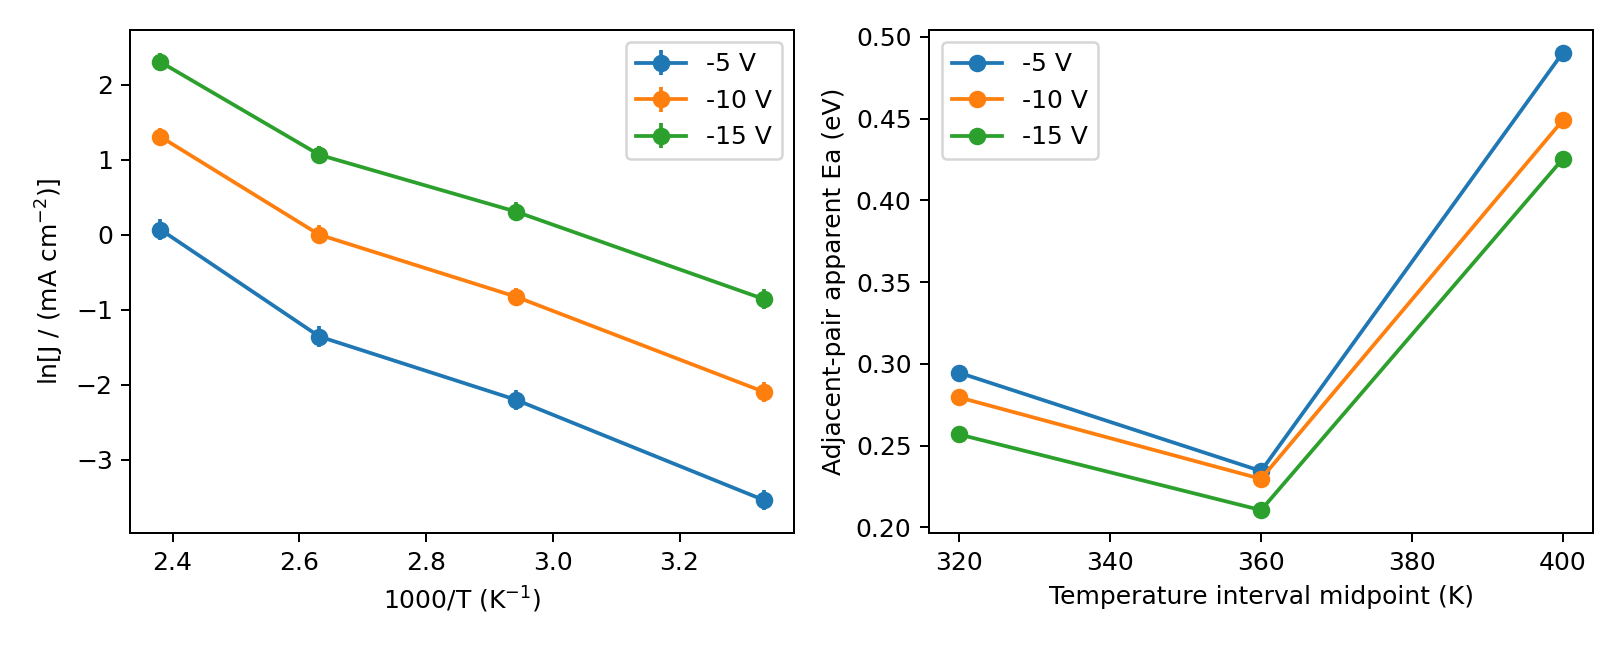
\includegraphics[width=.97\linewidth]{figures/S10_temperature_digitization.png}
\caption{S10 {\cjkfont 端电流的温度读图及曲率检查。固定的是端电压；该组器件厚度尚未核实，故不换算为固定局部电场。图中的误差来自指定像素包络。}\allowbreak{}}\label{fig:S10-temperature}
\end{figure}

\subsection{{\cjkfont 早期近欧姆接触控制与暴露的问题}\allowbreak{}}
{\cjkfont 示例使用}\allowbreak{} $\sigma_n=\sigma_p=0.1$ eV{\cjkfont 、}\allowbreak{}$a=1$ nm{\cjkfont 、}\allowbreak{}$N=10^{21}\,\mathrm{cm^{-3}}${\cjkfont ；}\allowbreak{}300 K {\cjkfont 零密度零场迁移率锚到旧基线，仅为受控比较。它们不是目标材料测量参数。所有温度共用参数，没有逐温度拟合。旧模型的态密度为}\allowbreak{} $10^{19}\,\mathrm{cm^{-3}}${\cjkfont ，故完整更换}\allowbreak{} DOS {\cjkfont 后的变化不能全归因于迁移率。}\allowbreak{}

{\cjkfont 已比较旧单能级恒迁移率、仅加入温度迁移率、}\allowbreak{}Gaussian DOS {\cjkfont 冻结迁移率，以及}\allowbreak{} Gaussian DOS {\cjkfont 与完整}\allowbreak{} $\mu(n,F,T)$ {\cjkfont 四组。单独输运示例在固定}\allowbreak{} $n=10^{16}\,\mathrm{cm^{-3}}${\cjkfont 、}\allowbreak{}$F=10^5\,\mathrm{V\,cm^{-1}}$ {\cjkfont 下，}\allowbreak{}420/300 K {\cjkfont 的迁移率比约为}\allowbreak{} 17.6{\cjkfont ；这一比值并不自动成为器件电流比。}\allowbreak{}

{\cjkfont 空间细化给出了决定性的警告：}\allowbreak{}300 K {\cjkfont 完整}\allowbreak{} Gaussian {\cjkfont 器件的}\allowbreak{} 161 {\cjkfont 到}\allowbreak{} 321 {\cjkfont 节点变化在已测反偏点不超过}\allowbreak{} 0.92\%{\cjkfont ，}\allowbreak{}420 K {\cjkfont 却仍变化}\allowbreak{} 43--45\%{\cjkfont 。因此粗网格完整器件的激活能和所谓}\allowbreak{}“{\cjkfont 迁移率使电流增加}\allowbreak{} 54--64\%”{\cjkfont 不再用于定量解释。}\allowbreak{}

420 K{\cjkfont 、}\allowbreak{}$-5$ V {\cjkfont 时，非局域净产生约}\allowbreak{} $0.504\,\mu\mathrm{A\,cm^{-2}}${\cjkfont 、双分子热产生约}\allowbreak{} $8.07\,\mu\mathrm{A\,cm^{-2}}$ {\cjkfont 已近稳定，但单端接触注入随细网格从}\allowbreak{} 2.84 {\cjkfont 增至}\allowbreak{} 7.58{\cjkfont 、再到}\allowbreak{} $16.6\,\mu\mathrm{A\,cm^{-2}}${\cjkfont 。接触占据约为三分之一，远超过低密度拟合窗；最大}\allowbreak{} $qFa/\sigma$ {\cjkfont 从}\allowbreak{} 1.69 {\cjkfont 增至}\allowbreak{} 3.39{\cjkfont 。由}\allowbreak{} DOS {\cjkfont 压缩率估算的屏蔽长度约}\allowbreak{} 0.25 nm{\cjkfont ，小于假设分子间距}\allowbreak{} 1 nm{\cjkfont 。继续把连续介质网格细化到亚分子尺度，不能解决物理模型的层级问题。}\allowbreak{}

{\cjkfont 冻结迁移率的接触控制在}\allowbreak{} 161{\cjkfont 、}\allowbreak{}321{\cjkfont 、}\allowbreak{}641 {\cjkfont 节点给出}\allowbreak{} 8.727{\cjkfont 、}\allowbreak{}8.786{\cjkfont 、}\allowbreak{}$8.820\,\mu\mathrm{A\,cm^{-2}}${\cjkfont ，末次变化}\allowbreak{} 0.386\%{\cjkfont 。这支持问题集中在未验证的接触输运闭合，但不能证明恒迁移率替代真实。}\allowbreak{}

{\cjkfont 已通过的检查包括模块积分、正反详细平衡、平衡零电流、通量符号、制造解空间收敛及保存状态的电荷}\allowbreak{}/{\cjkfont 电流}\allowbreak{}/{\cjkfont 能量核验。它们证明所写方程被一致处理，不证明参数已标定或所有器件预测均已收敛。}\allowbreak{}

\subsection{{\cjkfont 高占据微观边界基准与局限}\allowbreak{}}
{\cjkfont 为避免把低密度经验迁移率外推到接触高占据区，我们建立了一个独立的分子尺度边界基准。它包含}\allowbreak{} 8 {\cjkfont 个位点、全部}\allowbreak{} $2^8=256$ {\cjkfont 个排斥占据构型、}\allowbreak{}Gaussian {\cjkfont 随机裸能级、}\allowbreak{}Miller--Abrahams {\cjkfont 双向跳跃和有限速率双向电极交换。每条跃迁使用完整构型的能量差，而非只用平均占据的静电势。电子占据限制与相关性因此被显式保留。}\allowbreak{}

{\cjkfont 模型的固定电极势热力学势为}\allowbreak{}
\begin{equation}
 U(\boldsymbol n)=\sum_i n_i(\varepsilon_i-q\phi_{\mathrm{ext},i})+
 \frac{q^2a}{2\epsilon A}(\boldsymbol n-\boldsymbol b)^T
 L^{-1}(\boldsymbol n-\boldsymbol b).
\end{equation}
{\cjkfont 这里以焦耳计能量，}\allowbreak{}$L$ {\cjkfont 为无量纲}\allowbreak{} Dirichlet {\cjkfont 离散}\allowbreak{} Laplace {\cjkfont 矩阵，}\allowbreak{}$a=1$ nm{\cjkfont 、}\allowbreak{}$A=4$ nm$^2${\cjkfont ，电极间长度为}\allowbreak{} 9 nm{\cjkfont 。固定正补偿背景每站为}\allowbreak{} $b=0.3$ {\cjkfont 个元电荷。这是平面电容链的假想几何，不能当成三维分子之间精确的}\allowbreak{} $1/r$ {\cjkfont 势，也不是样品已知掺杂。电压源作用已经包含在构型势中，跃迁时不能再加第二份场做功。}\allowbreak{}

{\cjkfont 保持参数和无序不变，计算}\allowbreak{} 12 {\cjkfont 组无序、}\allowbreak{}4 {\cjkfont 个温度和}\allowbreak{} 2 {\cjkfont 个平均外加场，共}\allowbreak{} 96 {\cjkfont 个工况，另作}\allowbreak{} 26 {\cjkfont 个条件控制。已完成稳态概率、截面粒子流、正反详细平衡、}\allowbreak{}Gauss {\cjkfont 电荷和功热关系的核验及独立复核。这个系统只有一种载流子，没有电子}\allowbreak{}--{\cjkfont 空穴成对产生、复合或热失控。}\allowbreak{}

\begin{figure}[htbp]\centering
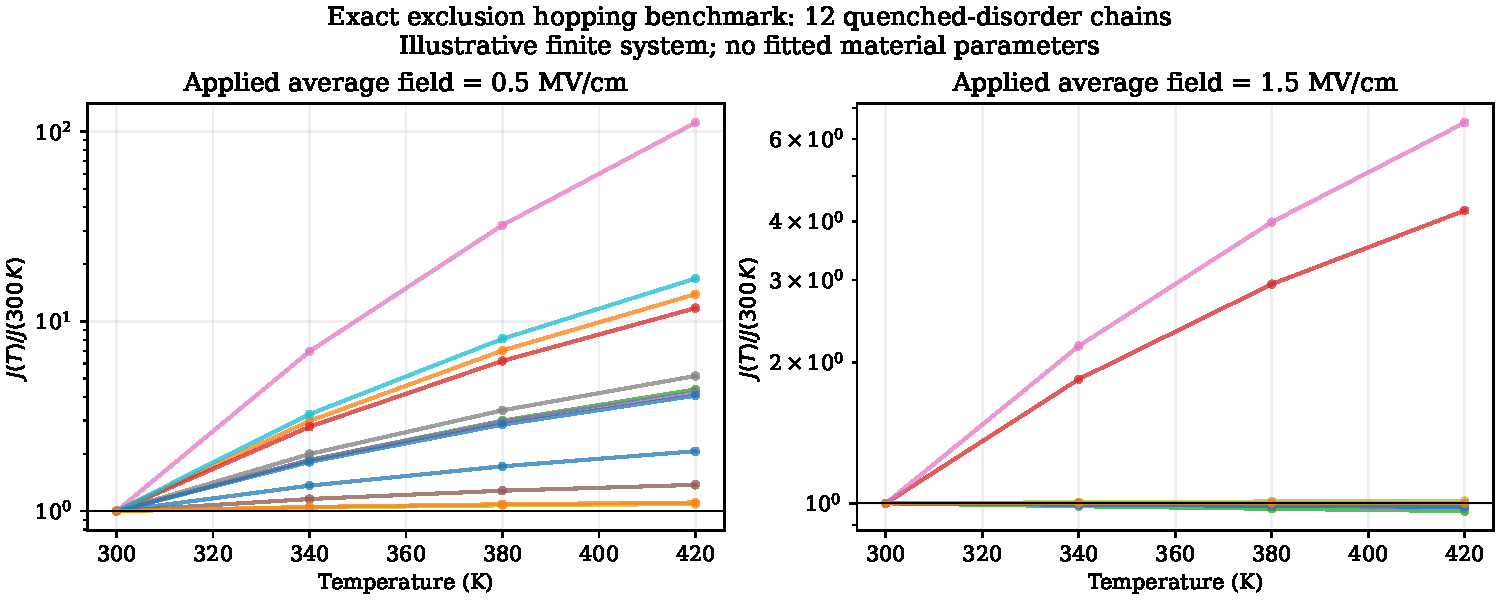
\includegraphics[width=.97\linewidth]{figures/temperature_exclusion_benchmark.pdf}
\caption{{\cjkfont 有限排斥跳跃链的温度反例。每条链电流幅值按自身}\allowbreak{} 300 K {\cjkfont 归一化；固定的是外加平均场。所有非温度参数均固定。它不是器件}\allowbreak{} J--V{\cjkfont ，也没有与实验电流幅值拟合。}\allowbreak{}}\label{fig:exclusion-temperature}
\end{figure}

{\cjkfont 在}\allowbreak{} $0.5\,\mathrm{MV\,cm^{-1}}$ {\cjkfont 下，各链的}\allowbreak{} $|J(420)|/|J(300)|$ {\cjkfont 从}\allowbreak{} 1.09 {\cjkfont 到}\allowbreak{} 111.6{\cjkfont ；在}\allowbreak{} $1.5\,\mathrm{MV\,cm^{-1}}$ {\cjkfont 下，}\allowbreak{}12 {\cjkfont 条链中有}\allowbreak{} 10 {\cjkfont 条落在}\allowbreak{} 0.9625--1.0115{\cjkfont ，另外两条为}\allowbreak{} 4.22 {\cjkfont 和}\allowbreak{} 6.51{\cjkfont 。纯跳跃也能给出几乎平坦、甚至略下降的端电流：高场使部分前向跃迁进入下坡速率上限，而逆向过程、占据和电极交换仍在变化。由此可严格否定}\allowbreak{}“{\cjkfont 弱温度依赖足以证明弹性隧穿}\allowbreak{}”{\cjkfont 这一单独判据；不能据样本比例判断宏观薄膜机制。}\allowbreak{}

{\cjkfont 这项反例也有明确假设。有效最近邻时钟取恒定}\allowbreak{} $10^9\,\mathrm{s^{-1}}${\cjkfont ，已吸收固定距离衰减，并非真实材料的温度无关前因子测量。关闭电容相互作用的排斥链仍可给出约}\allowbreak{} 0.955 {\cjkfont 的温度比，说明弱温度反例并不完全依赖补偿背景。然而保留充电而删除背景会引发极强阻塞，显著改变绝对电流。背景、电容和几何不能作为隐蔽的拟合自由度。}\allowbreak{}

\begin{figure}[htbp]\centering
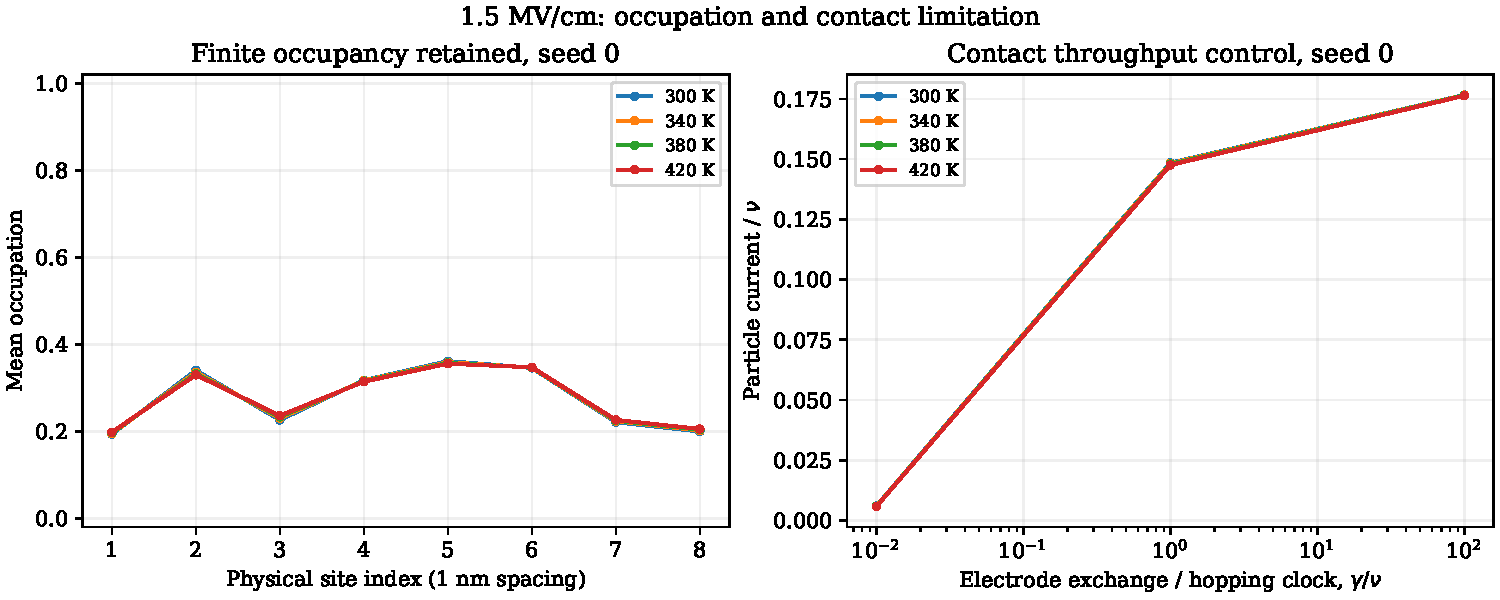
\includegraphics[width=.97\linewidth]{figures/contact_occupancy_controls.pdf}
\caption{{\cjkfont 微观接触控制展示交换速率、占据和充电假设的影响。改变位点数改变物理长度与无序片段，不是同一器件的数值网格细化。绝对电流由假定通道面积与时钟决定，不能与实际暗电流直接比较。}\allowbreak{}}\label{fig:contact-occupancy-control}
\end{figure}

{\cjkfont 该基准证明可在有限高占据系统中避免}\allowbreak{} EGDM {\cjkfont 外推，同时保留详细平衡与电荷守恒。它尚未修复前述}\allowbreak{} 100 nm {\cjkfont 器件，也没有建立三维无序平均或宏观尺寸收敛。下一步必须处理微观接触区与连续体体相的化学势、通量和电荷匹配，不能把有限链电流直接作为新的体产生率。}\allowbreak{}

\subsection{{\cjkfont 完整器件变温预测与接触条件}\allowbreak{}}
{\cjkfont 本轮进一步完成电子、空穴、}\allowbreak{}Poisson {\cjkfont 电势、高斯态密度、}\allowbreak{}$\mu(n,F,T)${\cjkfont 、非局域}\allowbreak{} Marcus {\cjkfont 产生与再俘获及双电极边界的联合稳态求解。温度取}\allowbreak{} 300{\cjkfont 、}\allowbreak{}340{\cjkfont 、}\allowbreak{}380{\cjkfont 、}\allowbreak{}420 K{\cjkfont ，反偏取}\allowbreak{} $-5${\cjkfont 、}\allowbreak{}$-10${\cjkfont 、}\allowbreak{}$-15$ V{\cjkfont 。每个接触情景的全部温度共用同一组参数。这建立了可复算的完整等温器件预测；结果仍没有重现文献温度幅度。}\allowbreak{}

{\cjkfont 为保留前述近欧姆接触的失败证据，本轮另设对称接触势垒}\allowbreak{} $b=0.4$ {\cjkfont 和}\allowbreak{} $0.5$ eV{\cjkfont 。能级排列一致规定}\allowbreak{} $V_{\rm bi}=(E_g-2b)/q${\cjkfont ，对应内建电压}\allowbreak{} 0.5 {\cjkfont 和}\allowbreak{} 0.3 V{\cjkfont 。提高多数载流子势垒的同时，反向少数载流子的互补势垒}\allowbreak{} $E_g-b$ {\cjkfont 降为}\allowbreak{} 0.9 {\cjkfont 和}\allowbreak{} 0.8 eV{\cjkfont ，因此反向注入会增强。这是两个不同的条件器件，不能称为原}\allowbreak{} $b=0.05$ eV {\cjkfont 器件的数值修复；本轮也没有沿用其}\allowbreak{} FF78 {\cjkfont 性能结论。}\allowbreak{}

{\cjkfont 共享条件为厚度}\allowbreak{} 100 nm{\cjkfont 、}\allowbreak{}$E_g=1.3$ eV{\cjkfont 、}\allowbreak{}$\epsilon_r=3.5${\cjkfont 、}\allowbreak{}$\sigma_n=\sigma_p=0.1$ eV{\cjkfont 、}\allowbreak{}$a=1$ nm{\cjkfont 、}\allowbreak{}$N=a^{-3}=10^{21}\,\mathrm{cm^{-3}}${\cjkfont ，}\allowbreak{}300 K {\cjkfont 零密度零场}\allowbreak{} $\mu_n=\mu_p=0.0045247\,\mathrm{cm^2\,V^{-1}\,s^{-1}}${\cjkfont 。产生中心取}\allowbreak{} $N_t=10^{15}\,\mathrm{cm^{-3}}${\cjkfont 、中隙能级、每支距离}\allowbreak{} 1 nm{\cjkfont 、}\allowbreak{}$H_0=1$ meV{\cjkfont 、}\allowbreak{}$\lambda=0.3$ eV{\cjkfont 、局域化长度}\allowbreak{} $\xi=0.5$ nm{\cjkfont ，两种方向平分中心数，有效反应厚度}\allowbreak{} 96 nm{\cjkfont 。它们都是条件参数，未作材料联合标定。}\allowbreak{}

{\cjkfont 反应使用经典高温}\allowbreak{} Marcus {\cjkfont 核并对两个高斯末态库积分，包含占据和空位因子；四速率满足详细平衡。它不是已经验证的}\allowbreak{} MLJ {\cjkfont 核，也不是对论文图}\allowbreak{} 2d {\cjkfont 路径的唯一识别。另有可逆双分子控制支路，固定}\allowbreak{} $\beta=10^{-11}\,\mathrm{cm^3\,s^{-1}}${\cjkfont ；该唯象参数不能直接称为已确定的}\allowbreak{} Langevin {\cjkfont 系数。固定补偿背景为}\allowbreak{} $N_t/2${\cjkfont ，不代表孤立中心具有半整数电荷。}\allowbreak{}

\begin{table}[htbp]\centering\small
\begin{tabular}{rrrrrr}\toprule
$b$ (eV)&$V$ (V)&300 K&340 K&380 K&420 K\\\midrule
0.4&$-5$&0.001459&0.06191&1.246&14.48\\
0.4&$-10$&0.005150&0.1869&3.359&35.69\\
0.4&$-15$&0.01717&0.5072&7.878&74.86\\
0.5&$-5$&0.06458&1.771&24.89&215.4\\
0.5&$-10$&0.2291&5.435&68.54&545.8\\
0.5&$-15$&0.7559&14.79&161.7&1154\\\bottomrule
\end{tabular}
\caption{{\cjkfont 完整器件的}\allowbreak{} $|J|${\cjkfont ，单位}\allowbreak{} $\mathrm{mA\,cm^{-2}}${\cjkfont ，}\allowbreak{}321 {\cjkfont 节点。高温大电流是外加恒温假设下的解；未计算自热和损伤，不能当作可安全维持的实验工作点。}\allowbreak{}}
\end{table}

\subsection{{\cjkfont 温度响应与文献不符之处}\allowbreak{}}
{\cjkfont 在固定端电压下，以四温度的}\allowbreak{} $\ln|J|$ {\cjkfont 对}\allowbreak{} $1/T$ {\cjkfont 拟合得到器件表观激活能。}\allowbreak{}$b=0.4$ eV {\cjkfont 的三个偏压对应}\allowbreak{} 0.8325{\cjkfont 、}\allowbreak{}0.8000{\cjkfont 、}\allowbreak{}0.7581 eV{\cjkfont ；}\allowbreak{}$b=0.5$ eV {\cjkfont 对应}\allowbreak{} 0.7339{\cjkfont 、}\allowbreak{}0.7033{\cjkfont 、}\allowbreak{}0.6630 eV{\cjkfont 。补充图}\allowbreak{} S10 {\cjkfont 的读图值为}\allowbreak{} 0.3140{\cjkfont 、}\allowbreak{}0.2972{\cjkfont 、}\allowbreak{}0.2757 eV{\cjkfont ，像素包络约}\allowbreak{} $\pm0.03$ eV{\cjkfont 。即使考虑这一读图不确定性，当前器件假设的温度依赖仍显著偏强。}\allowbreak{}

{\cjkfont 相应}\allowbreak{} $420/300$ K {\cjkfont 电流比，}\allowbreak{}$b=0.4$ eV {\cjkfont 为}\allowbreak{} 9925{\cjkfont 、}\allowbreak{}6929{\cjkfont 、}\allowbreak{}4359{\cjkfont ，}\allowbreak{}$b=0.5$ eV {\cjkfont 为}\allowbreak{} 3336{\cjkfont 、}\allowbreak{}2382{\cjkfont 、}\allowbreak{}1526{\cjkfont ；}\allowbreak{}S10 {\cjkfont 则约为}\allowbreak{} 36.9{\cjkfont 、}\allowbreak{}30.0{\cjkfont 、}\allowbreak{}23.6{\cjkfont 。一个常数幅值因子不能消除这些温度比的差异。比较使用端电压，因为}\allowbreak{} S10 {\cjkfont 厚度尚未核实；不能宣称是在相同局部电场下验证了某个核。四点也不严格满足单一}\allowbreak{} Arrhenius {\cjkfont 直线，拟合值仅是该温区的概括。}\allowbreak{}

\begin{figure}[htbp]\centering
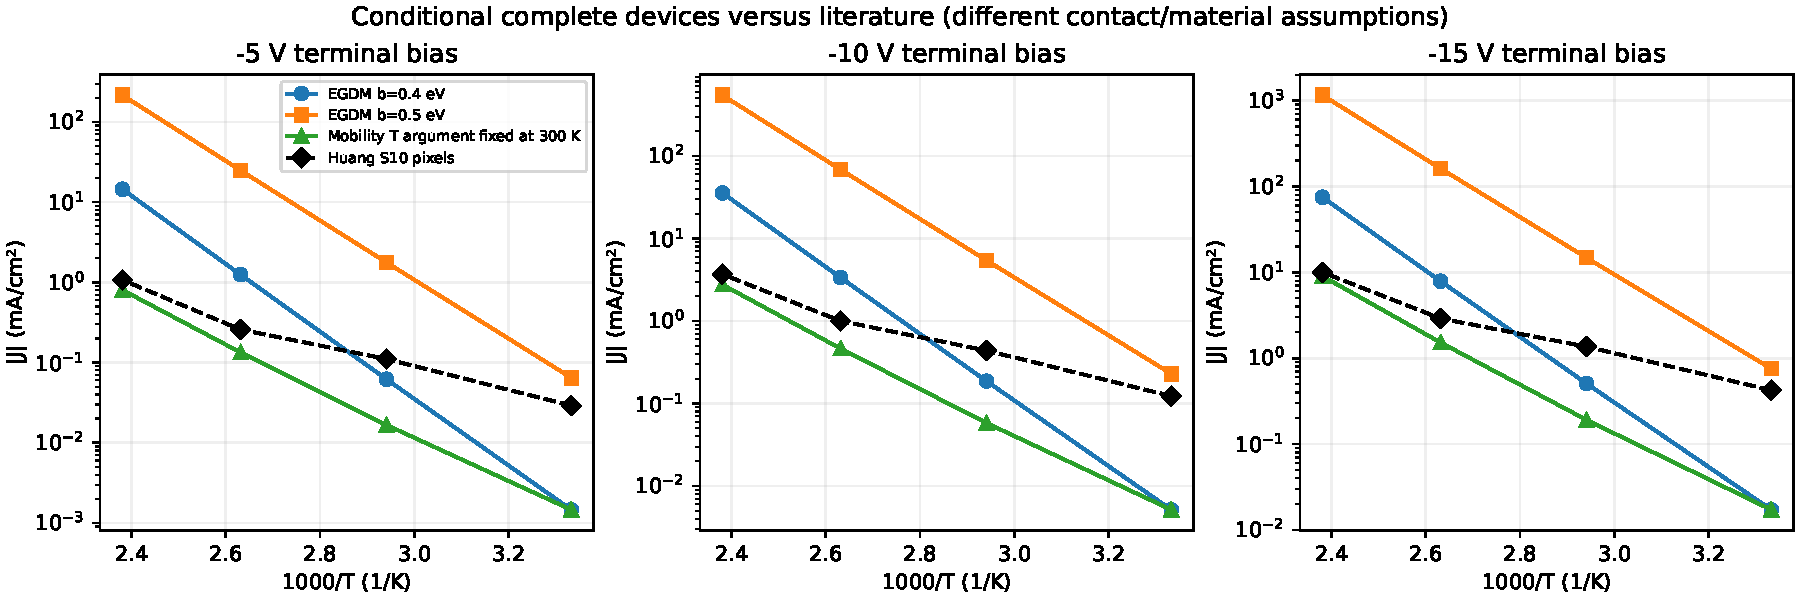
\includegraphics[width=.98\linewidth]{figures/temperature_device_comparison.pdf}
\caption{{\cjkfont 共享参数下完整器件与}\allowbreak{} Huang S10 {\cjkfont 读图对照。两个接触情景均具有过强的温度响应。文献点为数字化估计，模型线为等温条件预测；曲线不代表同一材料样品的拟合。}\allowbreak{}}
\end{figure}

\subsection{{\cjkfont 迁移率影响必须与电流来源同时分账}\allowbreak{}}
{\cjkfont 为辨认迁移率显式温度依赖的影响，控制计算只把}\allowbreak{} $\mu(n,F,T)$ {\cjkfont 中的温度参数固定为}\allowbreak{} 300 K{\cjkfont ，同时仍在实际温度下计算高斯占据、扩散热力学、反应核和接触供给。每一点重新联立求解，允许密度与场变化；这不是简单给端电流乘一个迁移率比，也不是另一种真实材料。}\allowbreak{}300 K {\cjkfont 的控制与完整模型严格相同。}\allowbreak{}

\begin{table}[htbp]\centering\small
\begin{tabular}{rrrrr}\toprule
$V$ (V)&$E_a$ {\cjkfont 完整}\allowbreak{}&$E_a$ {\cjkfont 冻结}\allowbreak{} $\mu$ {\cjkfont 温度}\allowbreak{}&420 K {\cjkfont 电流比}\allowbreak{}&$J_{\rm net\,gen}/|J|$\\\midrule
$-5$&0.8325&0.5699&18.07&$6.01\times10^{-4}$\\
$-10$&0.8000&0.5676&12.95&$2.86\times10^{-4}$\\
$-15$&0.7581&0.5659&8.30&$2.05\times10^{-4}$\\\bottomrule
\end{tabular}
\caption{$b=0.4$ eV {\cjkfont 的自洽控制。激活能单位}\allowbreak{} eV{\cjkfont ；电流比为完整模型除以只冻结迁移率显式温度的控制。最后一列在}\allowbreak{} 420 K {\cjkfont 比较净体产生折算电流与端电流。}\allowbreak{}}
\end{table}

{\cjkfont 这些情景的端电流远大于净体产生积分，说明主要是电极到电极泄漏。迁移率温度依赖确实显著影响端口响应，但拟合得到的激活能不能叫作陷阱发射势垒，也不能用来验证}\allowbreak{} Marcus {\cjkfont 产生主导。相反，在体产生受限且收集充分的极限，}\allowbreak{}$J\simeq q\int G\,dx${\cjkfont ，迁移率变化可以主要体现为密度与空间电荷调整，未必同幅改变端电流。两个极限必须由来源分账辨别。}\allowbreak{}

\begin{figure}[htbp]\centering
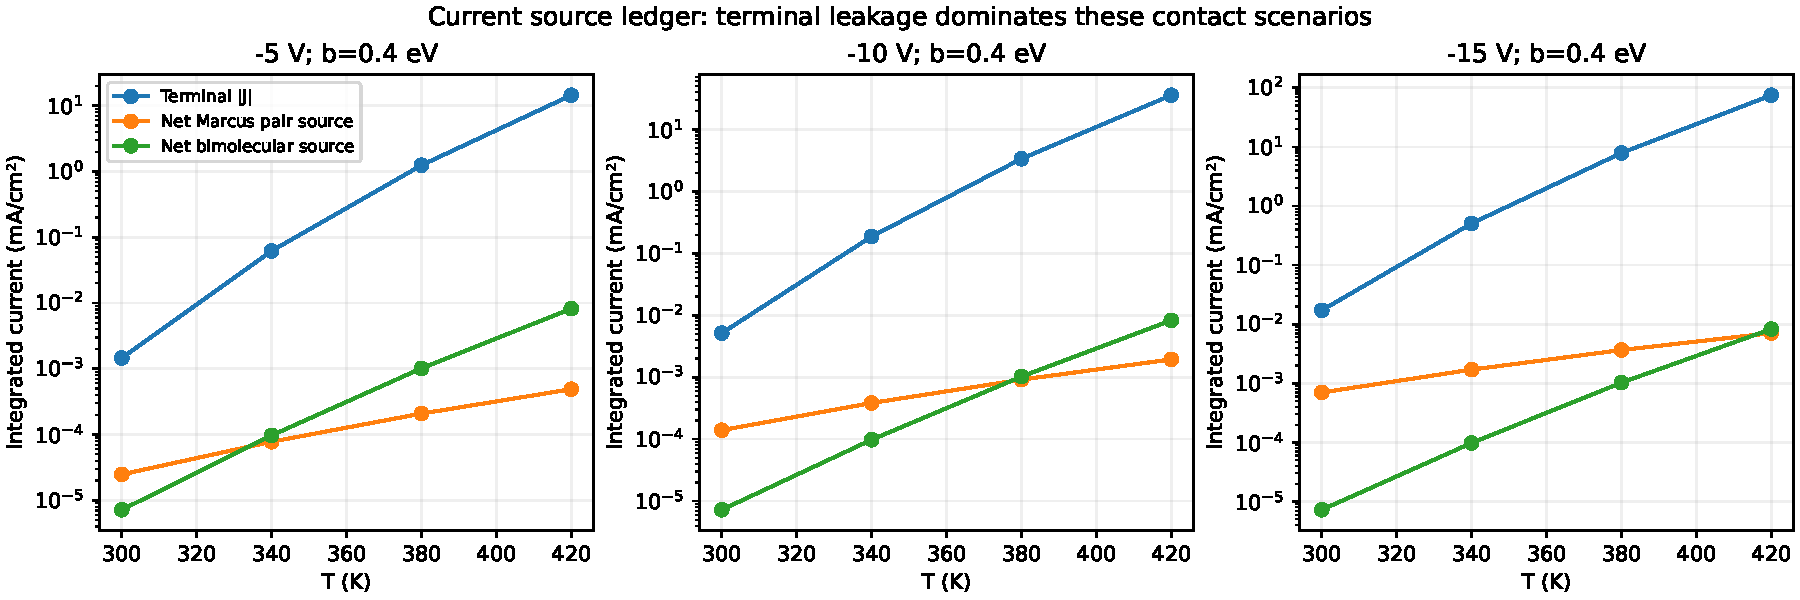
\includegraphics[width=.98\linewidth]{figures/source_current_ledger.pdf}
\caption{{\cjkfont 端电流、净产生与非局域源的温度分账。端电流明显大于体产生折算电流，支持本组条件下接触泄漏主导的判断。}\allowbreak{}}
\end{figure}

\subsection{{\cjkfont 独立材料参数与数值可信范围}\allowbreak{}}
Hosseini {\cjkfont 等在另一组}\allowbreak{} PM6:BTP-eC9 {\cjkfont 器件中由变温}\allowbreak{} SCLC {\cjkfont 与高斯无序模型报告：室温零场}\allowbreak{} $\mu_n=4.1\times10^{-4}${\cjkfont 、}\allowbreak{}$\mu_p=2.1\times10^{-4}\,\mathrm{cm^2\,V^{-1}\,s^{-1}}${\cjkfont ，}\allowbreak{}$\sigma_n=53${\cjkfont 、}\allowbreak{}$\sigma_p=60$ meV{\cjkfont 。该文}\allowbreak{} 80 nm {\cjkfont 厚度只属于其自己的样品，不能赋给}\allowbreak{} Huang S10{\cjkfont 。}\allowbreak{}Huang {\cjkfont 对应器件使用}\allowbreak{} PEDOT:PSS {\cjkfont 与}\allowbreak{} PFN-Br/Ag{\cjkfont ；用户暂定}\allowbreak{} D18:L8-BO {\cjkfont 与}\allowbreak{} PDINN{\cjkfont ，界面也不同。}\allowbreak{}

{\cjkfont 仅比较低密度零场温度项，本轮}\allowbreak{} 100 meV {\cjkfont 无序和系数}\allowbreak{} 0.42 {\cjkfont 给出}\allowbreak{} $\mu(420)/\mu(300)=21.72${\cjkfont ；独立文献的系数}\allowbreak{} 0.44 {\cjkfont 与}\allowbreak{} 53/60 meV {\cjkfont 则给出}\allowbreak{} 2.47/3.19{\cjkfont 。过强温度响应因此提示同时重新约束无序和接触。但直接将}\allowbreak{} 53/60 meV {\cjkfont 代入当前}\allowbreak{} EGDM {\cjkfont 全表达式，会使部分温区}\allowbreak{} $\sigma/k_BT<2${\cjkfont ，超出已确认的密度拟合窗；高场系数也尚未核验，不能无依据补齐。}\allowbreak{}

{\cjkfont 主情景的}\allowbreak{} 24 {\cjkfont 个温度与接触工况完成}\allowbreak{} 81{\cjkfont 、}\allowbreak{}161{\cjkfont 、}\allowbreak{}321 {\cjkfont 节点检查，后两者端电流最大变化}\allowbreak{} 0.2401\%{\cjkfont 。}\allowbreak{}420 K{\cjkfont 、}\allowbreak{}$b=0.4$ eV {\cjkfont 三个反偏点进一步细化到}\allowbreak{} 641 {\cjkfont 节点，较}\allowbreak{} 321 {\cjkfont 节点分别改变}\allowbreak{} 0.0626\%{\cjkfont 、}\allowbreak{}0.0802\%{\cjkfont 、}\allowbreak{}0.0932\%{\cjkfont ；冻结迁移率温度的}\allowbreak{} $-15$ V {\cjkfont 控制改变}\allowbreak{} 0.1569\%{\cjkfont 。包括平衡点和控制，共保存}\allowbreak{} 140 {\cjkfont 个状态。最短移动电荷热力学屏蔽长度约}\allowbreak{} 3.53 nm{\cjkfont ；本轮接触情景没有此前的高占据和高场越界，但适用域通过仍不等于材料验证。}\allowbreak{}

{\cjkfont 所有状态检查连续性、非局域内部电流、}\allowbreak{}Poisson {\cjkfont 电荷、正耗散与详细平衡；公共化学势下平衡净流和净产生为零。高斯积分从}\allowbreak{} 128 {\cjkfont 增至}\allowbreak{} 256 {\cjkfont 点的端电流变化约不超过}\allowbreak{} $2\times10^{-8}${\cjkfont ，但固定状态高阶连续性缺陷可略超过求解器}\allowbreak{} $10^{-8}$ {\cjkfont 门限，因此整体精度不能用迭代残差替代。网格误差以及更大的物理参数不确定性仍是主要限制。}\allowbreak{}

{\cjkfont 本轮完整等温预测与原近欧姆接触的失败对照应并列保留。下一步先约束输运和接触，再在同一基础上更换场增强产生机制。模型没有热方程、离子、热点或损伤变量，尚不预测真实不可逆击穿，也不将可逆膝点等同失效。}\allowbreak{}


\subsection{{\cjkfont 相同参数下的暗态正向检验}\allowbreak{}}
{\cjkfont 为检验上述反偏条件模型能否同时给出合理的另一极性响应，我们保持全部材料与接触参数不变，补算}\allowbreak{} 300{\cjkfont 、}\allowbreak{}340{\cjkfont 、}\allowbreak{}380{\cjkfont 、}\allowbreak{}420 K {\cjkfont 和两种接触情景的暗态正向曲线。电压从}\allowbreak{} 0 {\cjkfont 到}\allowbreak{} $+1.2$ V{\cjkfont ，步长}\allowbreak{} 0.05 V{\cjkfont ，共}\allowbreak{} 200 {\cjkfont 个稳态（含}\allowbreak{} 8 {\cjkfont 个平衡态）。正电压降低平衡内建电势落差；零偏净流为零，正向电流与正的端口耗散一致。没有为正偏或单个温度重新拟合参数。}\allowbreak{}

\textbf{{\cjkfont 高电流支路的限制。}\allowbreak{}}{\cjkfont 模型没有串联电阻、有限接触供给或热方程，并强制薄膜保持外加温度。精化后的}\allowbreak{} $b=0.4$ eV{\cjkfont 、}\allowbreak{}420 K{\cjkfont 、}\allowbreak{}$+1.2$ V {\cjkfont 给出约}\allowbreak{} $1175.53\,\mathrm{A\,cm^{-2}}${\cjkfont ，对应}\allowbreak{} $1410.64\,\mathrm{W\,cm^{-2}}${\cjkfont 。这一结果暴露了理想边界与等温近似的现实限制，不能解释为真实器件可维持的工作状态。数值收敛不等于物理预测可信。}\allowbreak{}

\begin{figure}[htbp]\centering
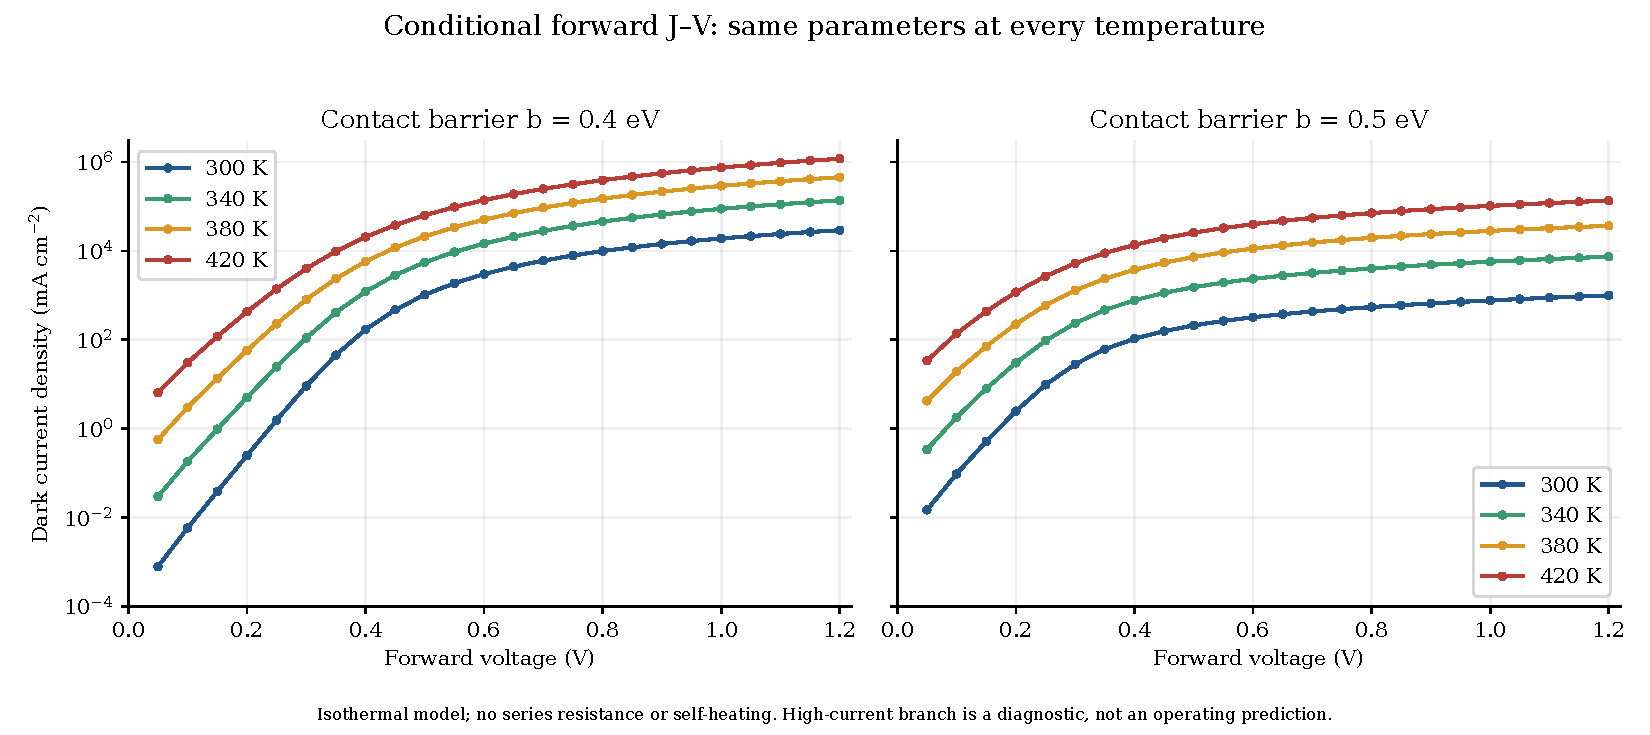
\includegraphics[width=.98\linewidth]{figures/forward_temperature_JV.pdf}
\caption{{\cjkfont 相同参数下的八条暗态正向温度曲线，主图采用}\allowbreak{} 161 {\cjkfont 节点。高正偏部分为无串联电阻和无自热反馈的理想方程诊断，不能当作真实工作电流。这里没有光照，不能计算太阳能电池的}\allowbreak{} FF {\cjkfont 或效率。}\allowbreak{}}
\end{figure}

\begin{table}[htbp]\centering\small
\begin{tabular}{rrrrrr}\toprule
$b$ (eV)&$V$ (V)&300 K&340 K&380 K&420 K\\\midrule
0.4&$+0.1$&$5.879\times10^{-6}$&$1.842\times10^{-4}$&0.003028&0.03059\\
0.4&$+0.3$&0.009136&0.1102&0.8034&3.984\\
0.4&$+0.5$&1.030&5.545&21.12&63.08\\
0.5&$+0.1$&$9.624\times10^{-5}$&0.001818&0.01948&0.1385\\
0.5&$+0.3$&0.02829&0.2365&1.298&5.241\\
0.5&$+0.5$&0.2109&1.527&7.275&25.65\\\bottomrule
\end{tabular}
\caption{{\cjkfont 暗态正向代表点的}\allowbreak{} $J${\cjkfont ，单位}\allowbreak{} $\mathrm{A\,cm^{-2}}${\cjkfont 。与前文反偏表的毫安单位不同；这些数值属于条件模型，尚无同样品变温正向数据逐点验证。}\allowbreak{}}
\end{table}

{\cjkfont 在}\allowbreak{} $b=0.4$ eV {\cjkfont 情景，}\allowbreak{}420/300 K {\cjkfont 电流比从}\allowbreak{} $+0.1$ V {\cjkfont 的约}\allowbreak{} 5203 {\cjkfont 变为}\allowbreak{} $+0.3$ V {\cjkfont 的}\allowbreak{} 436{\cjkfont 、}\allowbreak{}$+1.0$ V {\cjkfont 的}\allowbreak{} 39.3{\cjkfont ；四温度表观激活能相应约为}\allowbreak{} 0.774{\cjkfont 、}\allowbreak{}0.550{\cjkfont 、}\allowbreak{}0.332 eV{\cjkfont 。这种电压依赖包含输运、接触供给、空间电荷和复合的共同变化，不能直接读成一个陷阱深度。}\allowbreak{}

200 {\cjkfont 点通过电流、电荷、能量与四速率详细平衡检查。四个代表工况进一步作}\allowbreak{} 161{\cjkfont 、}\allowbreak{}321{\cjkfont 、}\allowbreak{}641 {\cjkfont 节点比较，后两者电流最大变化}\allowbreak{} 0.134\%{\cjkfont ，}\allowbreak{}161 {\cjkfont 到}\allowbreak{} 641 {\cjkfont 最大变化}\allowbreak{} 0.519\%{\cjkfont ；并非全部}\allowbreak{} 200 {\cjkfont 点都做过三网格检验。两代表点将高斯积分从}\allowbreak{} 128 {\cjkfont 增至}\allowbreak{} 256 {\cjkfont 阶，端电流变化分别为}\allowbreak{} $3.83\times10^{-10}$ {\cjkfont 和}\allowbreak{} $1.21\times10^{-11}${\cjkfont 。最高节点占据约}\allowbreak{} $6.14\times10^{-4}${\cjkfont ，最大约化场}\allowbreak{} $qFa/\sigma=0.151${\cjkfont ，没有高占据或高场外推。}\allowbreak{}

{\cjkfont 正向曲线构成相同条件参数的额外一致性检验，尚没有配套的同材料、同温度暗态正向文献数据进入比较。结合反偏}\allowbreak{} S10 {\cjkfont 的温度差距，它要求今后同时约束接触、无序、迁移率和串联电阻；不能只调一个电阻降低正向电流而忽略反偏。这里不报告光照}\allowbreak{} $V_{\rm oc}${\cjkfont 、}\allowbreak{}$J_{\rm sc}${\cjkfont 、}\allowbreak{}FF {\cjkfont 或效率，也不沿用旧}\allowbreak{} FF78 {\cjkfont 值。}\allowbreak{}


\subsection{{\cjkfont 接下来如何比较产生与接触机制}\allowbreak{}}
{\cjkfont 第一步是使接触和体输运各自处于可解释的范围，保留}\allowbreak{} Gaussian DOS{\cjkfont 、占据统计、扩散及局部场反馈的一致性。不能用无依据的迁移率截断掩盖高场外推，也不能改变注入势垒把曲线凑到}\allowbreak{} S10{\cjkfont 。}\allowbreak{}

{\cjkfont 第二步，在相同温度、厚度、无序和接触参数下，只更换有明确状态定义的产生循环，逐一报告每步速率、净产生、复合损失、接触净供给和端电流。对非局域转移还应保留两端源项与相应内部电流；不能把微观净跨窗电流再当成本地产生重复加入。}\allowbreak{}

{\cjkfont 第三步，以端口}\allowbreak{} $J(V,T)$ {\cjkfont 检查文献对应，同时把局域产生的温度导数与收集、输运、接触的贡献分开。室温仍是当前基线；低温用于后续区分机制，但需要同时检查跳跃参数化和局域准平衡的适用性。}\allowbreak{}

{\cjkfont 本章支持采用无序跳跃输运作为共同起点，尚不支持宣布}\allowbreak{} PF{\cjkfont 、}\allowbreak{}Marcus/MLJ{\cjkfont 、陷阱辅助隧穿或接触路线中的任何一条已被实验证实。模型之间最有价值的比较，是同样严格的守恒与参数约束下，哪些路线能够同时解释幅值、温度、厚度和接触改变，哪些路线在完整循环或边界处失败。}\allowbreak{}

\subsection{{\cjkfont 本章主要来源}\allowbreak{}}
\begin{enumerate}
\item Pasveer et al., Unified Description of Charge-Carrier Mobilities in Disordered Semiconducting Polymers, Physical Review Letters 94, 206601 (2005). \url{https://doi.org/10.1103/PhysRevLett.94.206601}.
\item Roichman and Tessler, Generalized Einstein relation for disordered semiconductors. \url{https://arxiv.org/abs/cond-mat/0109432}.
\item Doan, Glitzky and Liero, WIAS Preprint 2493 (2018). \url{https://doi.org/10.20347/WIAS.PREPRINT.2493}. {\cjkfont 本章参考其无序输运热力学闭合和逆活度离散。}\allowbreak{}
\item Huang et al., Perovskite--organic tandem solar cells with superior reverse-bias stability, Nature Materials (2026). \url{https://doi.org/10.1038/s41563-026-02541-6}. {\cjkfont 本章温度数据来自补充图}\allowbreak{} S10{\cjkfont ，不能与损坏阈值}\allowbreak{} $V_{\rm RB}$ {\cjkfont 混为同一观测量。}\allowbreak{}
\item Hosseini et al., Advanced Energy Materials (2023). \url{https://doi.org/10.1002/aenm.202203576}. {\cjkfont 独立器件的变温输运参数，不作为目标样品的已标定输入。}
\item Miller and Abrahams, Physical Review 120, 745 (1960). \url{https://doi.org/10.1103/PhysRev.120.745}. {\cjkfont 有限链采用其上坡热激活、下坡固定时钟的速率形式。}\allowbreak{}
\item Novikov, Hopping transport of interacting carriers in disordered organic materials. \url{https://arxiv.org/abs/0708.4313}. {\cjkfont 参考其对相互作用和动态相关的讨论；本章未复现该文的材料计算。}\allowbreak{}
\end{enumerate}
\FloatBarrier
\clearpage

